\subsection{Visualization}
\begin{figure*}
    \centering
    \includegraphics[width=1\textwidth]{all_embeddings_subplot_copy.png}
    \caption{Visualizations of datasets with known hierarchical structure; (d) and (s) correspond to generated deep and shallow hierarchies, respectively. Multiclass noise in generated data is depicted in gray.}
    \label{fig:panel-fig}
\end{figure*}
Visualizations of text embeddings colored by top-level categories appear in Figure \ref{fig:panel-fig}. The generated hierarchies with 25\% noise are visualized. PHATE and PCA are better able to separate the noise class as compared with t-SNE and UMAP, but PHATE better preserves noise semantics by its centralized location, indicating a relation with multiple classes. PCA and t-SNE plots are globally quite similar, but t-SNE provides more class discriminability. PHATE, by contrast, displays top-level categories as extremal points of the embedding and provides cleaner class separation than PCA and t-SNE. UMAP collapses most of the information onto a single dimension in some cases and in others bears similarity to PHATE although compressing points and, in some cases, shattering the global structure. Additional visualizations with default parameter settings for UMAP and PHATE are provided in the appendices in Figure \ref{fig:default-visuals}.

The trajectory of topics and themes in the visualizations can be analyzed in several different ways. We visualize how the sub-themes within the Ecosystems data transition between the two themes of "Economic Impact Metrics" and "Social Conflict Intensity" (Figure \ref{fig:ecosystems-trajectory}). Similarly with the Fisheries data, we use the specific concepts to determine how some of the sub-themes mapped between the categories of "Offshore Energy Infrastructure Development," "Marine Environmental Quality," and "Fish Population Metrics" (Figure \ref{fig:fisheries-trajectory}). We, furthermore, curate semantic trajectories in the Web of Science embedding on the basis of keywords associated to each data point as provided in the dataset (Figure \ref{fig:WoS-trajectory}). Lastly, we use the information at the docket level for the EPA data to determine thematic changes over space (Figure \ref{fig:epa-trajectory}). 

\begin{figure*}
    \centering 
\begin{subfigure}{0.48\textwidth}
    \centering
    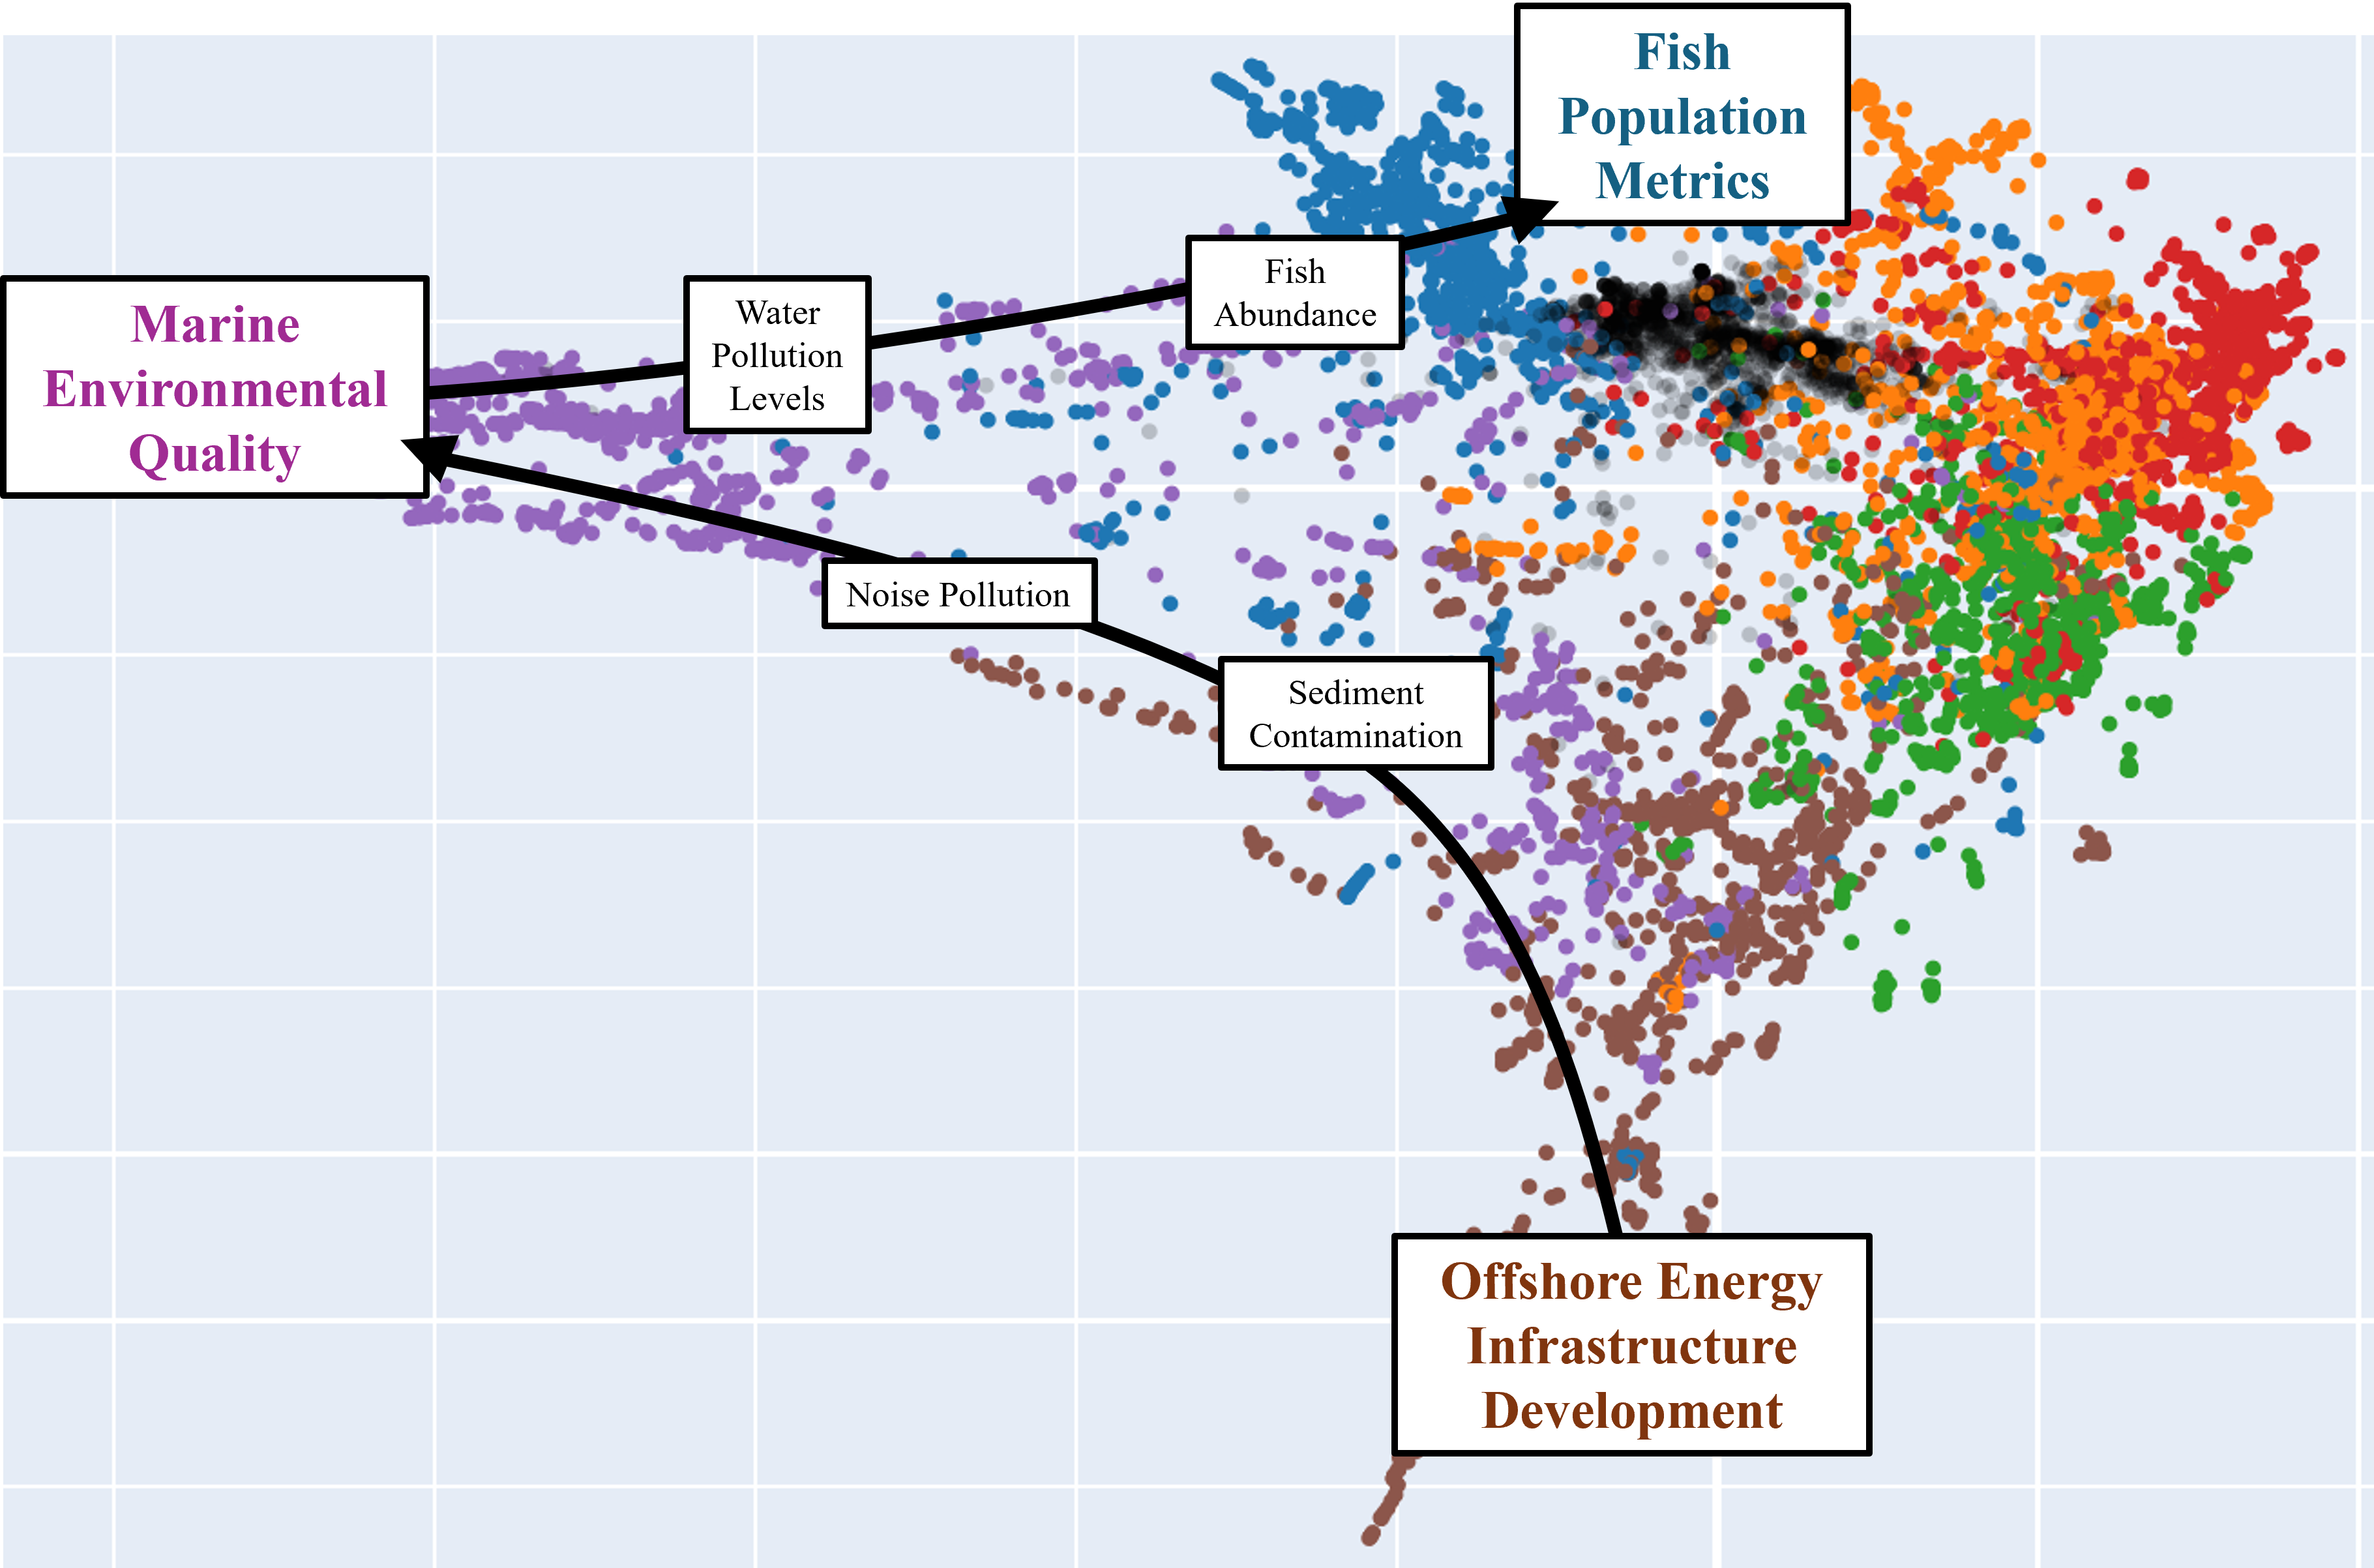
\includegraphics[width=\linewidth]{fisheries_trajectory.png}
    \caption{Trajectories in deep fisheries hierarchy}
    \label{fig:fisheries-trajectory}
\end{subfigure}
\begin{subfigure}{0.48\textwidth}
    \centering
    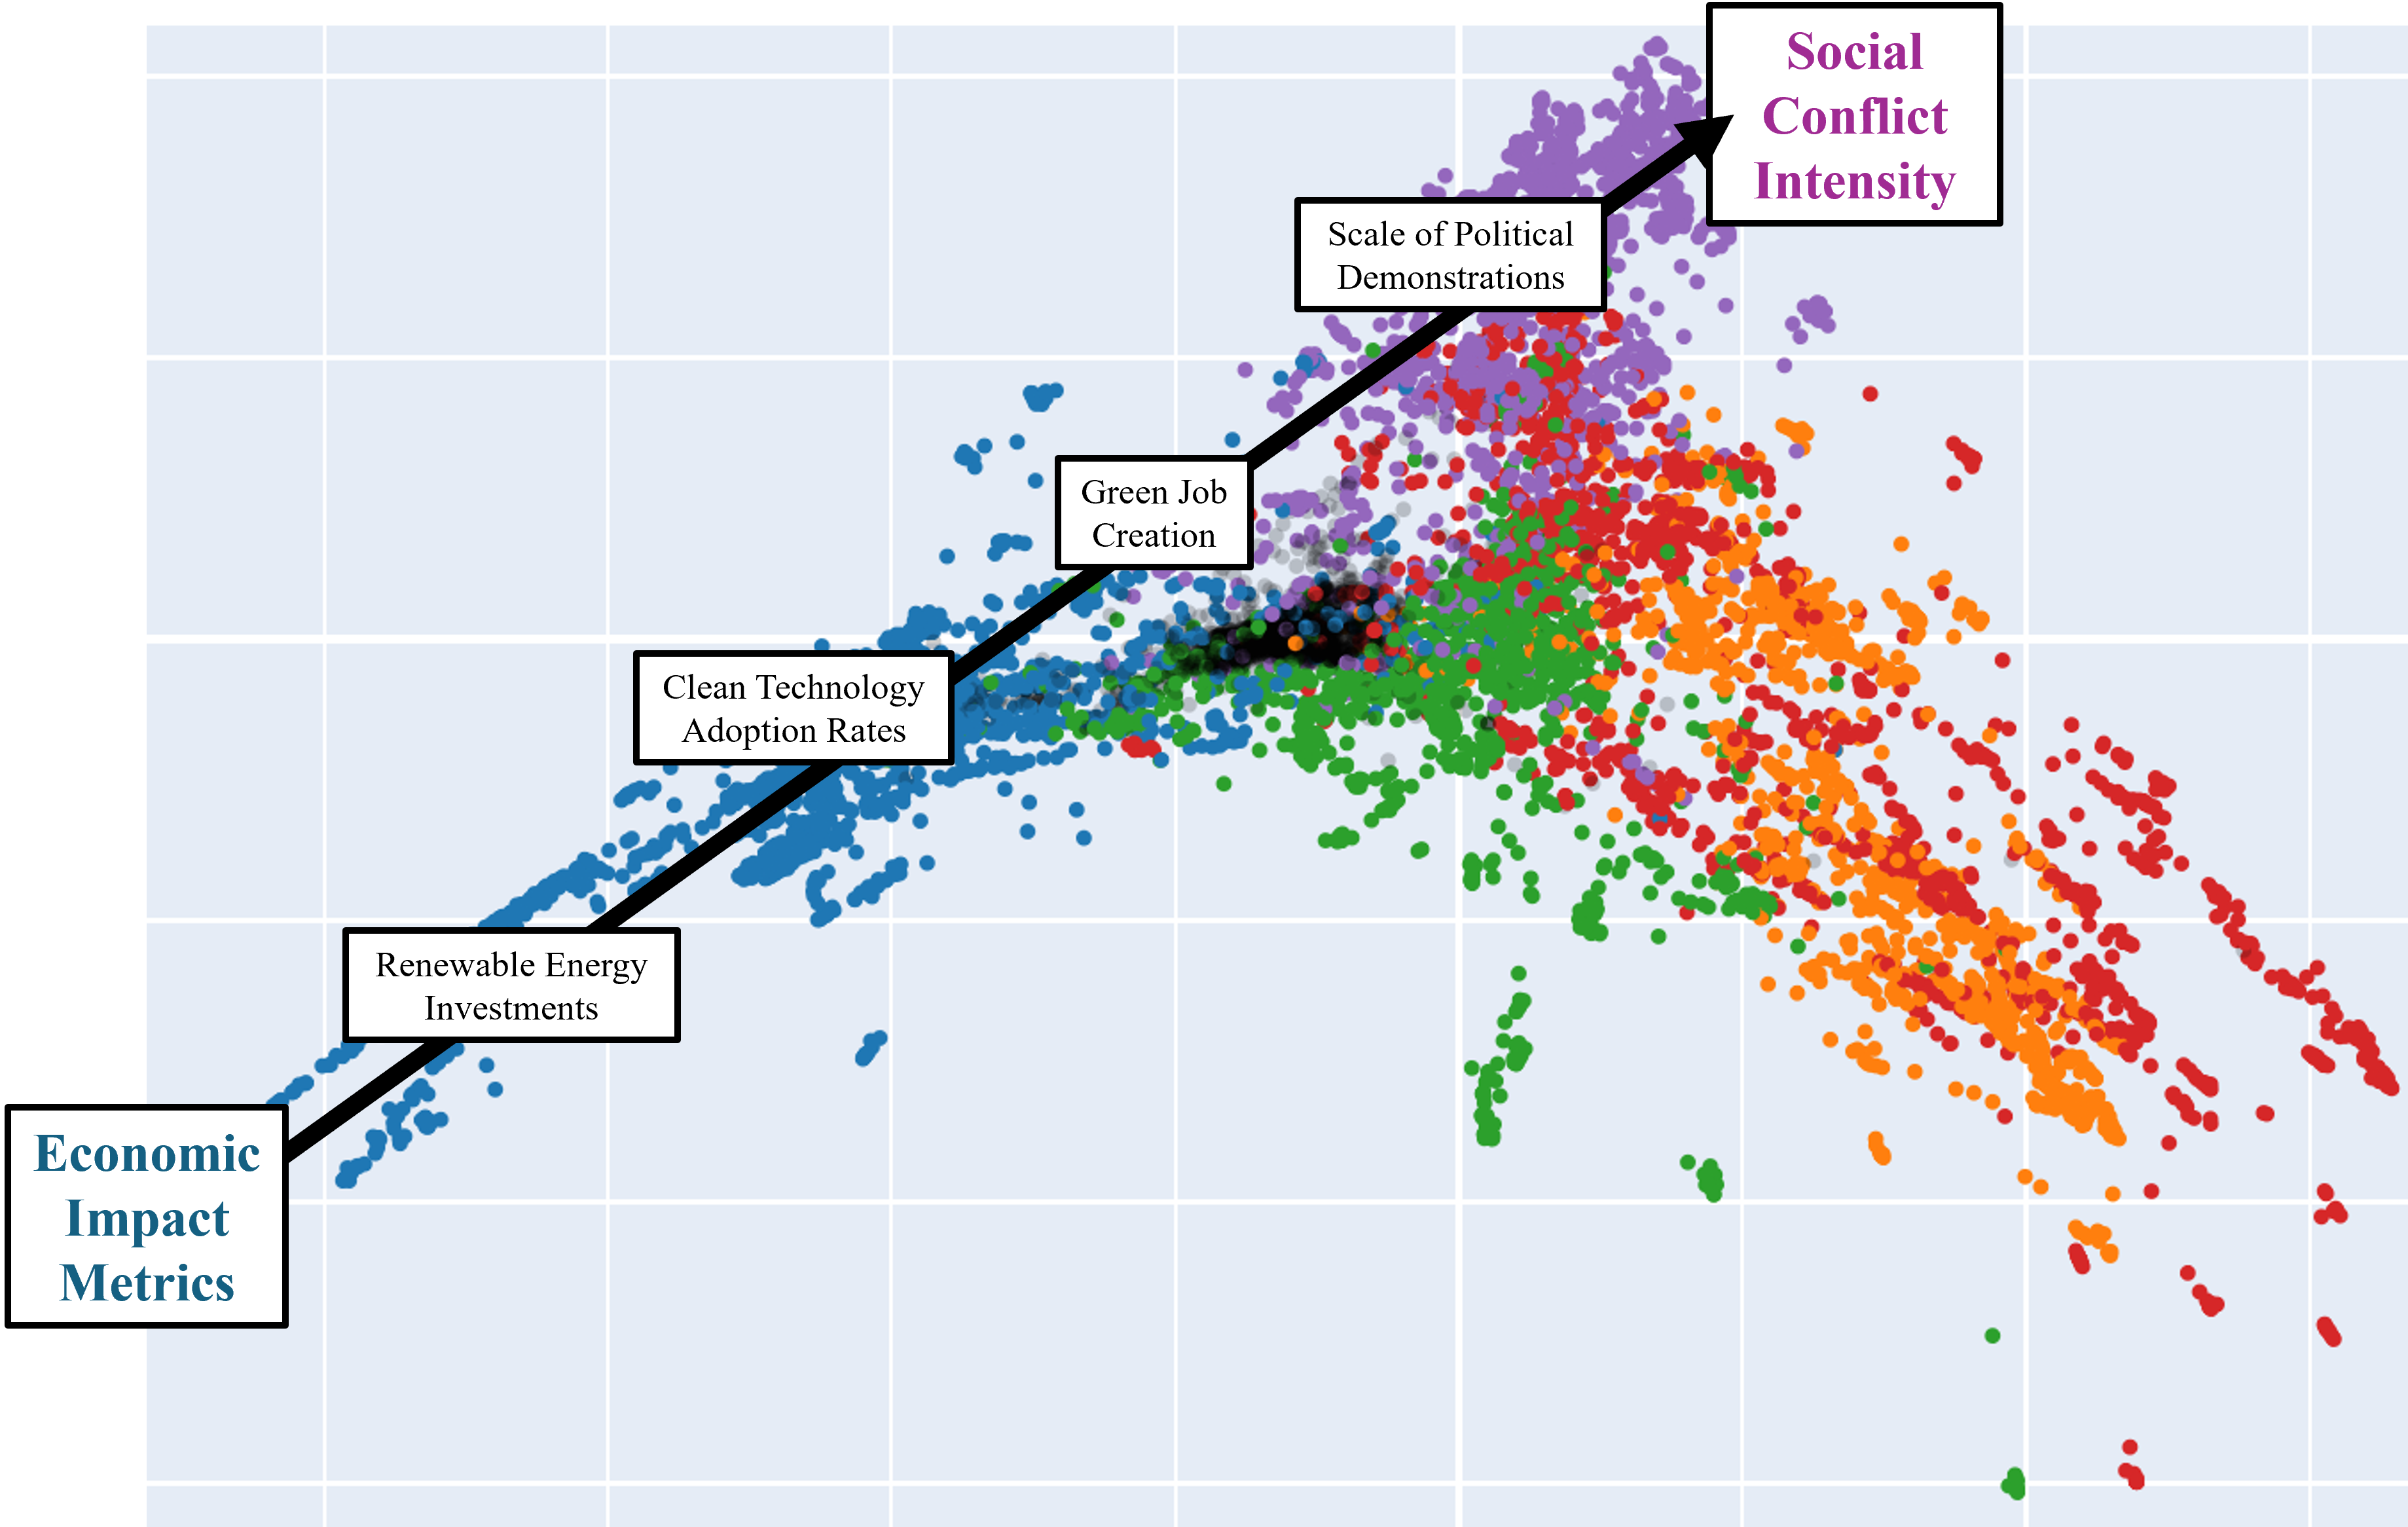
\includegraphics[width=\linewidth]{ecosystems_trajectory.png}
    \caption{Trajectories in deep ecosystems hierarchy}
    \label{fig:ecosystems-trajectory}
\end{subfigure}
\caption{"Narrative arc" trajectories in PHATE embedding space}
\label{fig:hierachy_trajectories}
\end{figure*}

\begin{figure*}
    \centering
    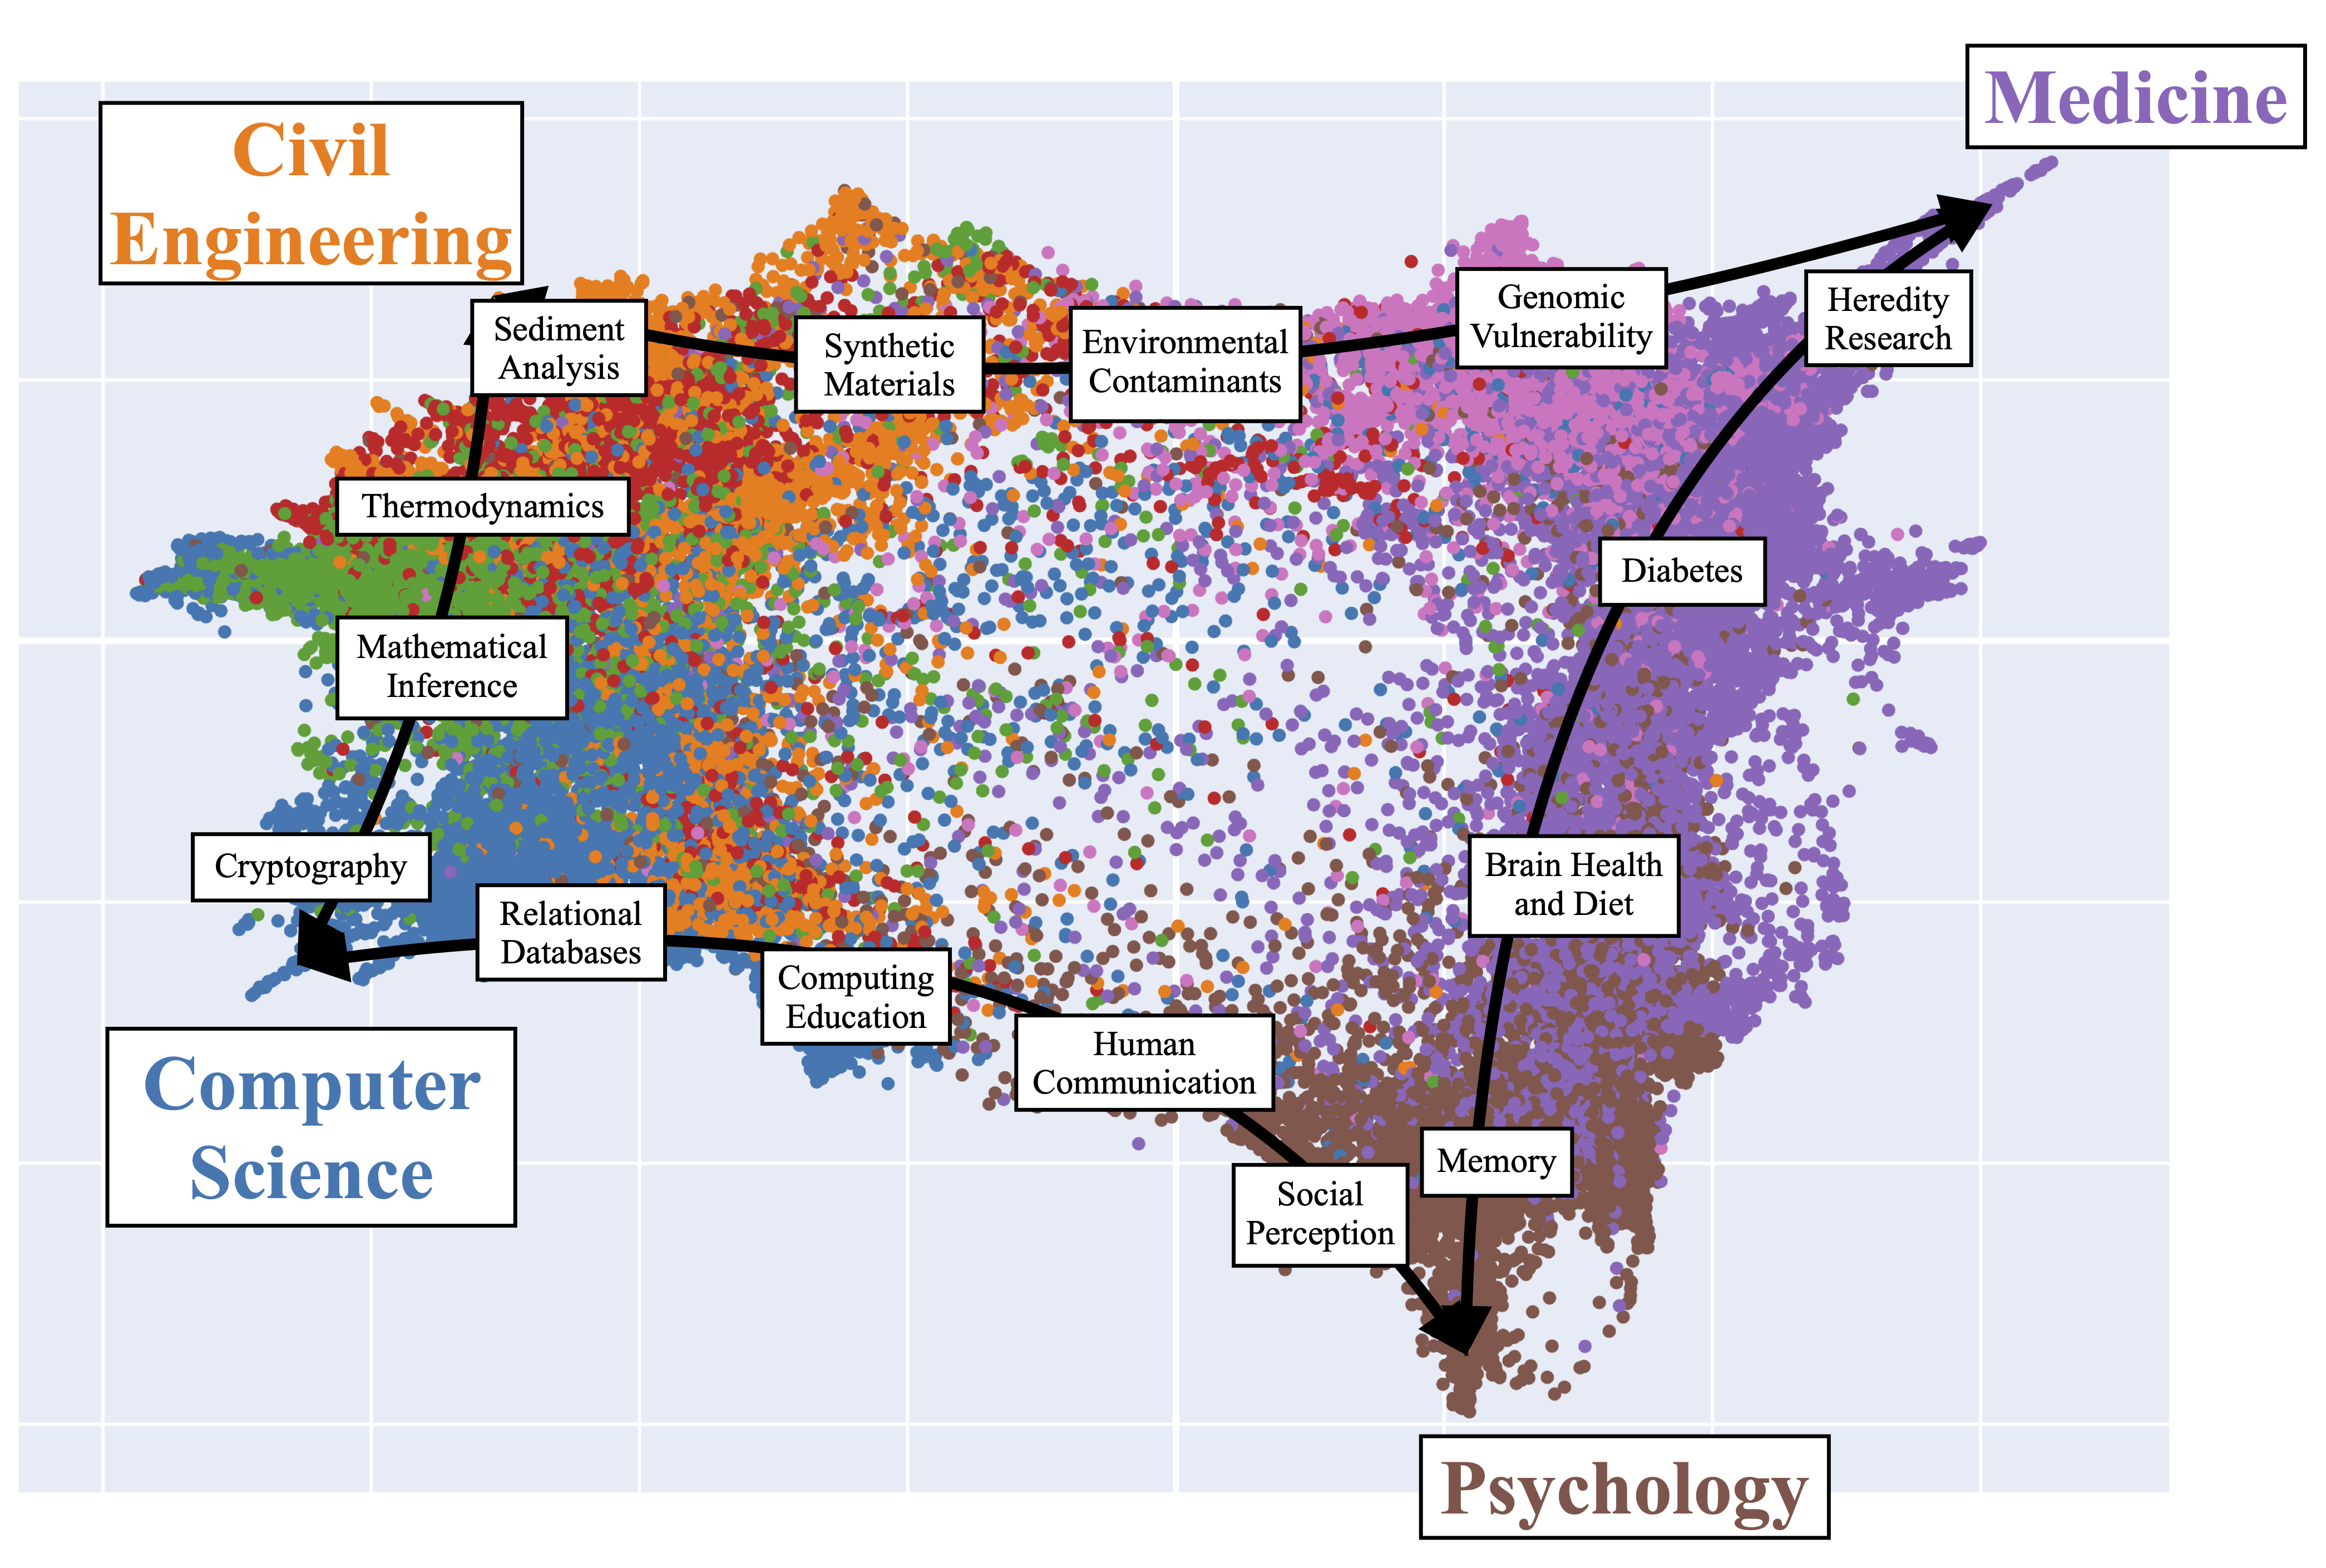
\includegraphics[width=1\linewidth]{phate_WOS.png}
    \caption{"Narrative arc" trajectories in PHATE embedding space of Web of Science}
    \label{fig:WoS-trajectory}
\end{figure*}  

\begin{figure}
    \centering
    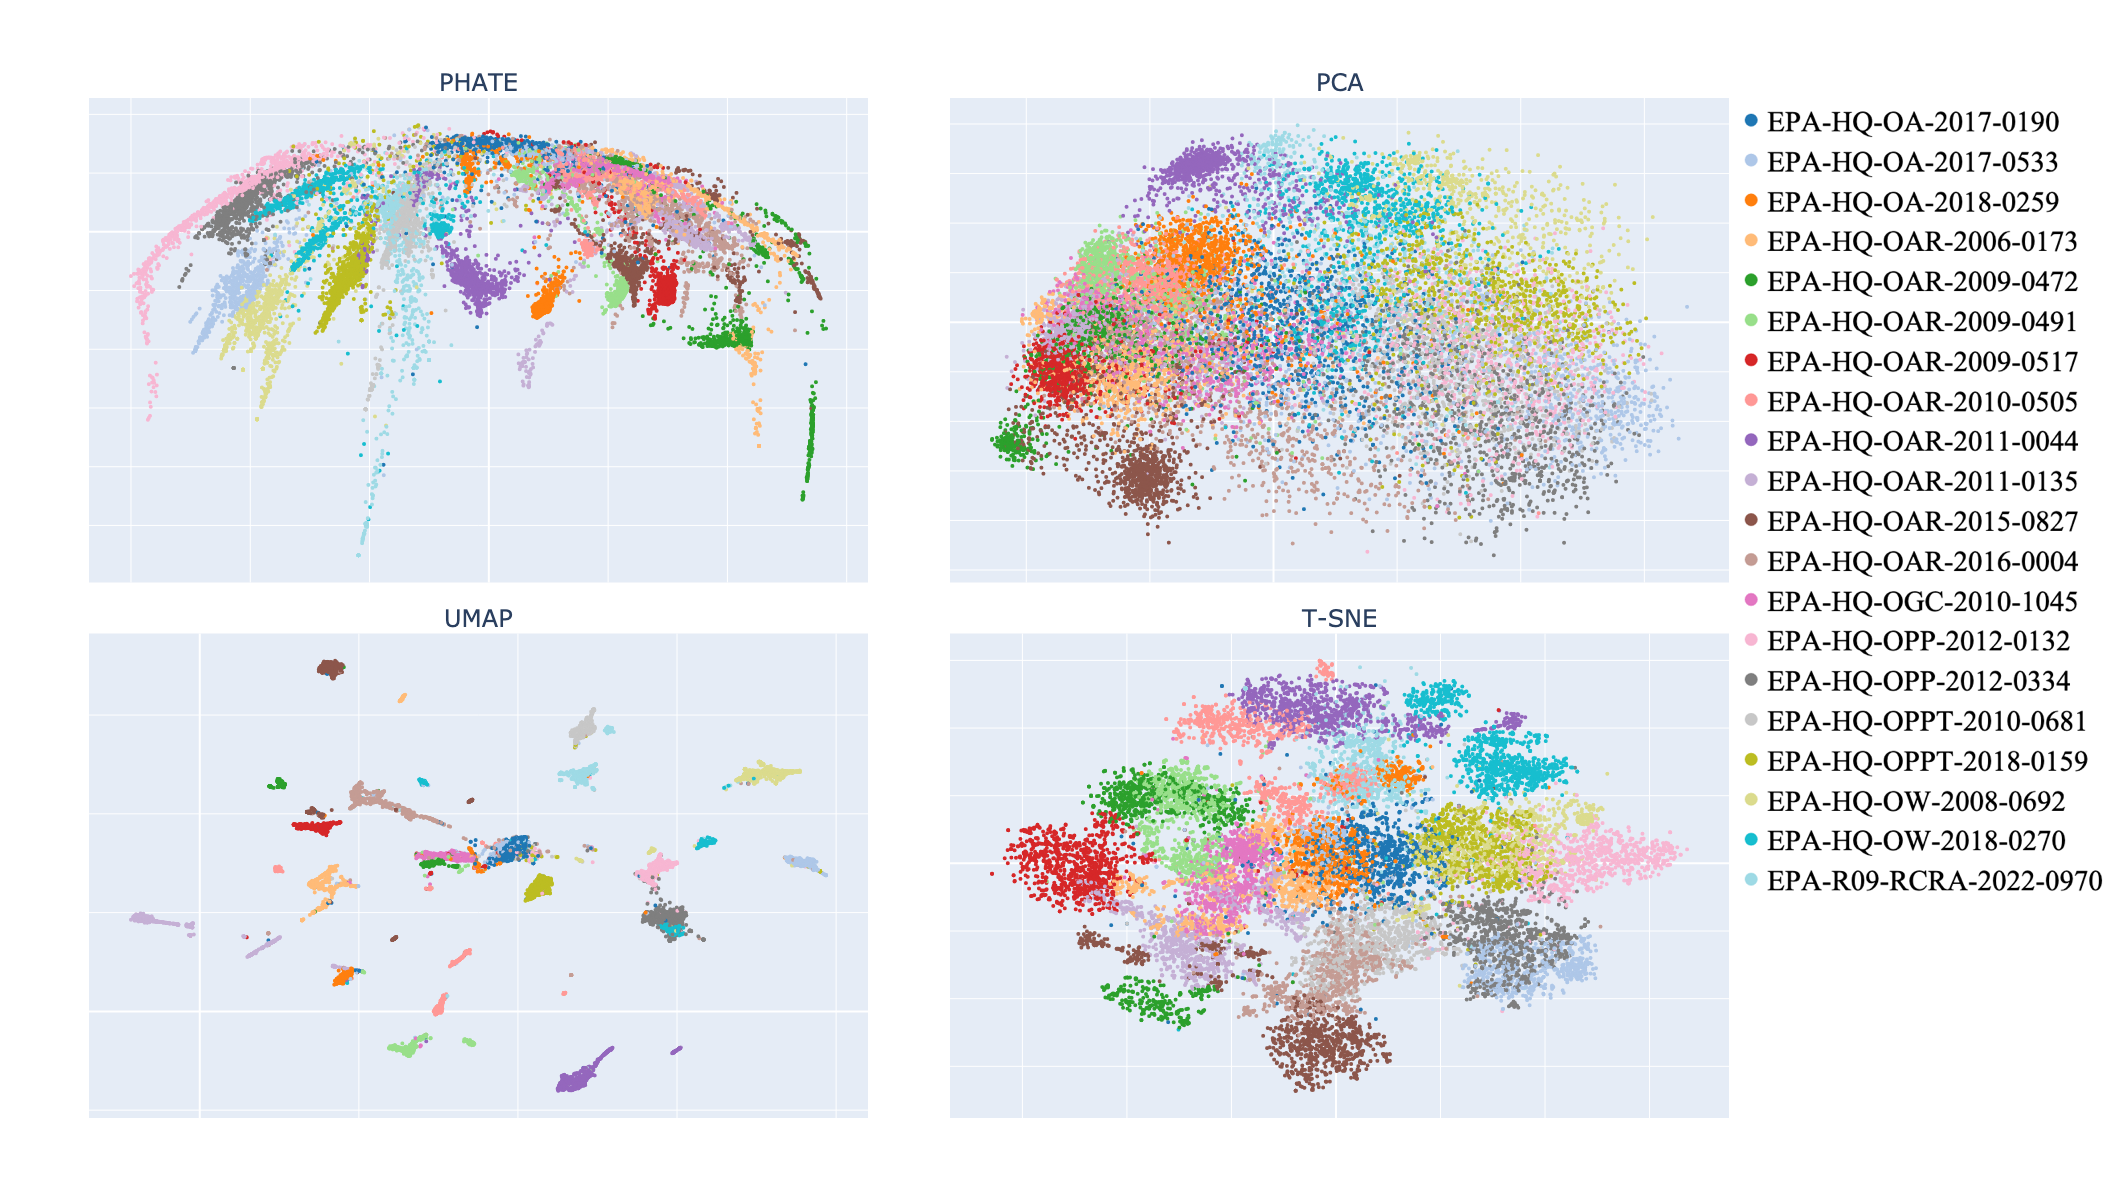
\includegraphics[width=1\linewidth]{epa_fig.png}
    \caption{Visualizations of head-tail embeddings of EPA comments colored by docket}
    \label{fig:epa-fig}
\end{figure}

\begin{figure}
    \centering
    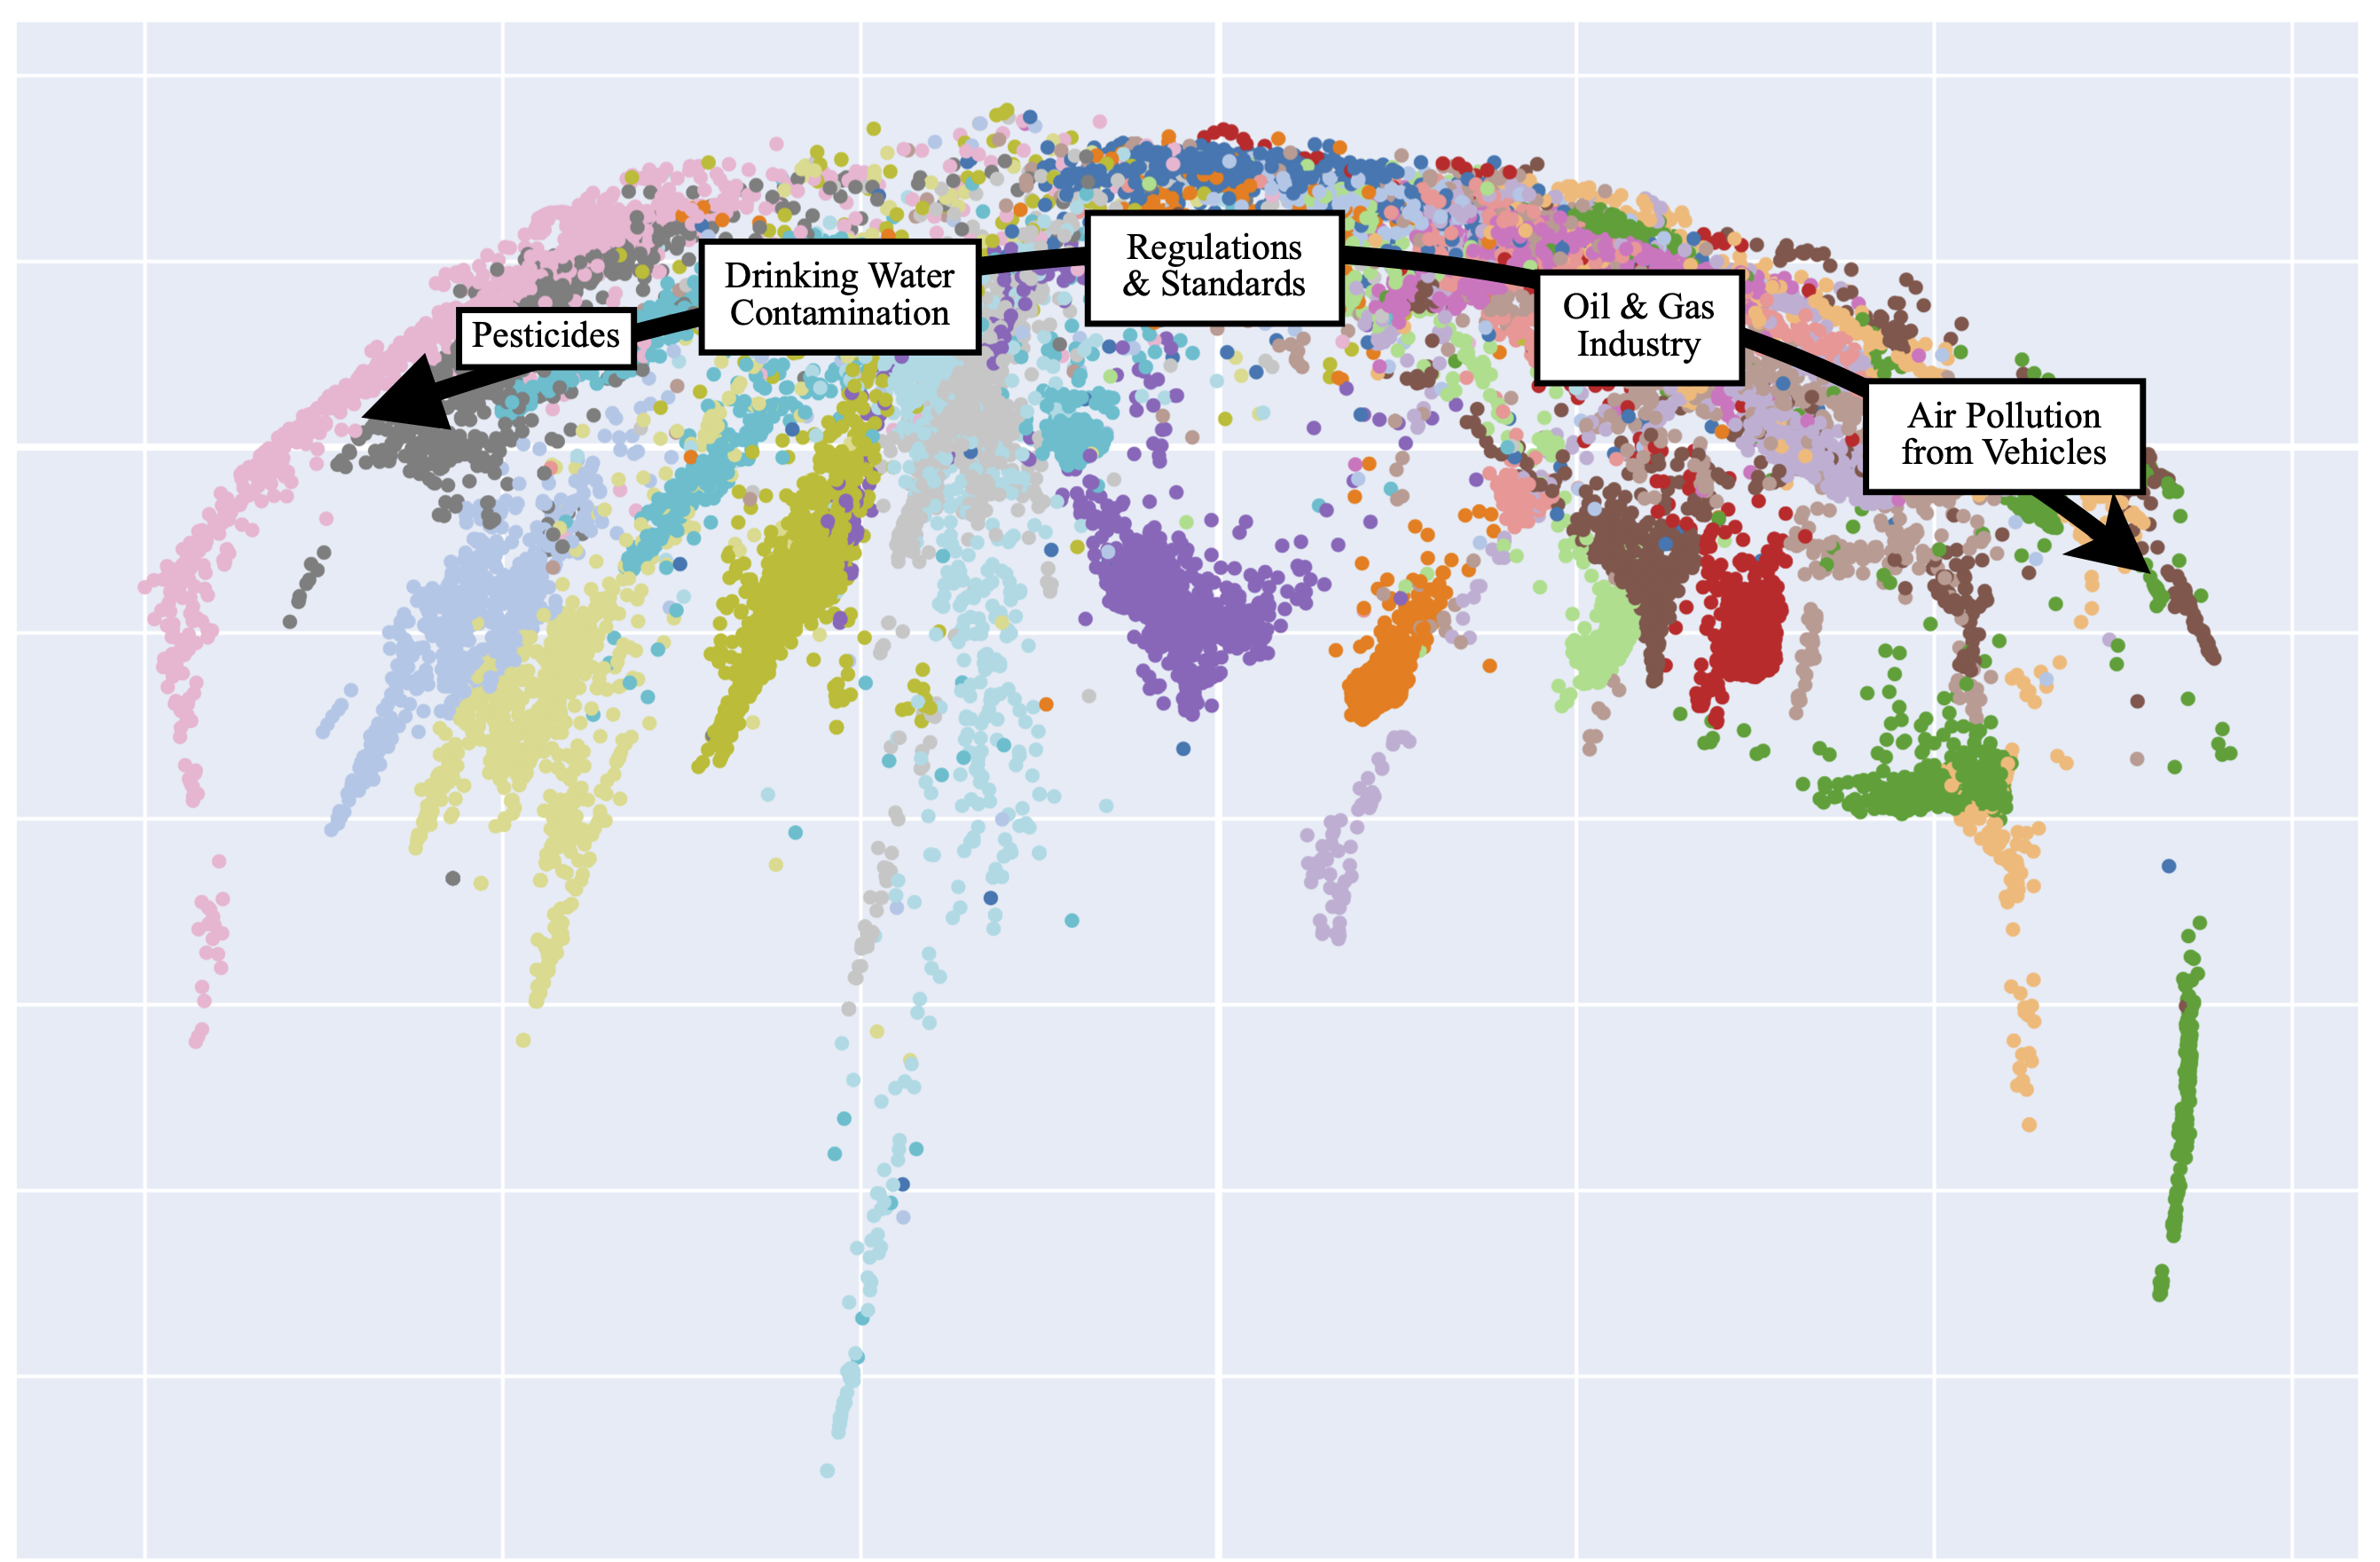
\includegraphics[width=1\linewidth]{epa_trajectory.png}
    \caption{"Narrative arc" trajectories in PHATE embedding space of EPA comments}
    \label{fig:epa-trajectory}
\end{figure}  

The visualization of PHATE compared to PCA, t-SNE and UMAP colored by the top 20 dockets is shown in Figure \ref{fig:epa-fig}. While PCA produces a dense and overlapping projection with limited visible structure, and t-SNE and UMAP highlight isolated clusters with distorted global relationships, PHATE preserves both local and global geometry using branching structures which suggest underlying transitions in comment themes across EPA dockets.
\FloatBarrier
\subsection{Dimensionality Reduction Evaluation}

As shown in Tables \ref{tab:dr_metrics} and \ref{tab:dr_synthetic}, across all datasets, including both synthetic benchmarks and real-world datasets such as arXiv and RCV1, trustworthiness and continuity values are consistently high, particularly for UMAP and PaCMAP. This indicates strong preservation of local neighborhood structure, with non-linear methods outperforming PCA and PHATE.

Shepard diagrams show deviation from the diagonal across all methods, indicating that global distances are not perfectly preserved. This suggests that dimensionality reduction introduces non-linear distortion, where distances are compressed in some regions and expanded in others.

Spearman rank correlation and DEMaP metrics further confirm moderate preservation of global structure. UMAP and PaCMAP achieve higher values across most datasets, while PCA consistently shows lower global structure preservation. These trends are consistent across datasets.

Overall, UMAP demonstrates the most consistent performance across both local and global metrics, with PaCMAP as a strong alternative, while PCA and PHATE show comparatively weaker performance.
% Real world dataset table
\begin{table*}[t]
    \centering
    \caption{Dimensionality reduction evaluation across datasets using trustworthiness, continuity, Spearman correlation, and DEMaP.}
\label{tab:dr_metrics}
    \begin{tabular}{llcccc}
    \toprule
    Dataset & Method & Trustworthiness & Continuity & Spearman & DEMaP \\
    \midrule
    RCV1 & PCA & 0.7781 & 0.8913 & 0.3965 & 0.4687 \\
    RCV1 & UMAP & 0.9563 & 0.9442 & 0.4863 & 0.6847 \\
    RCV1 & PHATE & 0.7979 & 0.9035 & 0.3725 & 0.6453 \\
    RCV1 & PaCMAP & 0.9360 & 0.9333 & 0.4218 & 0.6514 \\
    \midrule
    arXiv & PCA & 0.7606 & 0.8832 & 0.4858 & 0.4665 \\
    arXiv & UMAP & 0.9414 & 0.9290 & 0.5430 & 0.6406 \\
    arXiv & PHATE & 0.7988 & 0.8971 & 0.5796 & 0.6243 \\
    arXiv & PaCMAP & 0.9051 & 0.9274 & 0.5784 & 0.6442 \\
    \midrule
    Amazon & PCA & 0.7399 & 0.8523 & 0.3708 & 0.3605 \\
    Amazon & UMAP & 0.9164 & 0.9152 & 0.4400 & 0.5482 \\
    Amazon & PHATE & 0.7776 & 0.8833 & 0.4184 & 0.5123 \\
    Amazon & PaCMAP & 0.8645 & 0.8992 & 0.3964 & 0.4788 \\
    \midrule
    DBpedia & PCA & 0.7116 & 0.8563 & 0.3095 & 0.2374 \\
    DBpedia & UMAP & 0.9706 & 0.9371 & 0.2967 & 0.5000 \\
    DBpedia & PHATE & 0.8087 & 0.9068 & 0.2244 & 0.4385 \\
    DBpedia & PaCMAP & 0.9353 & 0.9325 & 0.2585 & 0.4501 \\
    \midrule
    WoS & PCA & 0.7866 & 0.8850 & 0.5444 & 0.5760 \\
    WoS & UMAP & 0.9504 & 0.9434 & 0.5313 & 0.7099 \\
    WoS & PHATE & 0.8505 & 0.9207 & 0.5438 & 0.7024 \\
    WoS & PaCMAP & 0.9102 & 0.9434 & 0.5289 & 0.6892 \\
    \bottomrule
    \end{tabular}
\end{table*}

% synthetic dataset (clean + noise)
\begin{table*}[t]
    \centering
    \caption{Dimensionality reduction evaluation on synthetic hierarchical datasets (depth3 and depth5) under varying noise conditions.}
    \label{tab:dr_synthetic}
    \begin{tabular}{lllcccc}
    \toprule
    Dataset & Condition & Method & Trustworthiness & Continuity & Spearman & DEMaP \\
    \midrule
    
    % ================= Ecosystem d3 =================
    Ecosystem (d3) & Clean & PCA & 0.8920 & 0.9173 & 0.3365 & 0.4121 \\
    Ecosystem (d3) & Clean & UMAP & 0.9490 & 0.9307 & 0.4535 & 0.6623 \\
    Ecosystem (d3) & Clean & PHATE & 0.9142 & 0.9251 & 0.4012 & 0.6154 \\
    Ecosystem (d3) & Clean & PaCMAP & 0.9401 & 0.9284 & 0.4328 & 0.6489 \\
    
    Ecosystem (d3) & 25\% Noise & PCA & 0.8851 & 0.9102 & 0.2987 & 0.3652 \\
    Ecosystem (d3) & 25\% Noise & UMAP & 0.9449 & 0.9348 & 0.3935 & 0.5851 \\
    Ecosystem (d3) & 25\% Noise & PHATE & 0.9023 & 0.9214 & 0.3422 & 0.5520 \\
    Ecosystem (d3) & 25\% Noise & PaCMAP & 0.9365 & 0.9299 & 0.3715 & 0.5903 \\
    
    Ecosystem (d3) & 50\% Noise & PCA & 0.8798 & 0.9043 & 0.2756 & 0.3310 \\
    Ecosystem (d3) & 50\% Noise & UMAP & 0.9425 & 0.9397 & 0.4246 & 0.6430 \\
    Ecosystem (d3) & 50\% Noise & PHATE & 0.8967 & 0.9188 & 0.3121 & 0.5104 \\
    Ecosystem (d3) & 50\% Noise & PaCMAP & 0.9312 & 0.9345 & 0.3524 & 0.5632 \\
    
    % ================= Ecosystem d5 =================
    Ecosystem (d5) & Clean & PCA & 0.9053 & 0.9281 & 0.3982 & 0.4720 \\
    Ecosystem (d5) & Clean & UMAP & 0.9678 & 0.9590 & 0.5081 & 0.6610 \\
    Ecosystem (d5) & Clean & PHATE & 0.9264 & 0.9412 & 0.4410 & 0.6302 \\
    Ecosystem (d5) & Clean & PaCMAP & 0.9551 & 0.9510 & 0.4725 & 0.6527 \\
    
    Ecosystem (d5) & 25\% Noise & PCA & 0.8987 & 0.9214 & 0.2874 & 0.3621 \\
    Ecosystem (d5) & 25\% Noise & UMAP & 0.9632 & 0.9571 & 0.3038 & 0.4220 \\
    Ecosystem (d5) & 25\% Noise & PHATE & 0.9175 & 0.9350 & 0.2711 & 0.4012 \\
    Ecosystem (d5) & 25\% Noise & PaCMAP & 0.9498 & 0.9486 & 0.2984 & 0.4150 \\
    
    Ecosystem (d5) & 50\% Noise & PCA & 0.8920 & 0.9158 & 0.2645 & 0.3318 \\
    Ecosystem (d5) & 50\% Noise & UMAP & 0.9568 & 0.9547 & 0.3187 & 0.4419 \\
    Ecosystem (d5) & 50\% Noise & PHATE & 0.9102 & 0.9321 & 0.2833 & 0.3987 \\
    Ecosystem (d5) & 50\% Noise & PaCMAP & 0.9450 & 0.9442 & 0.3012 & 0.4301 \\
    
    % ================= Fisheries d3 =================
    Fisheries (d3) & Clean & PCA & 0.8815 & 0.9043 & 0.3220 & 0.4015 \\
    Fisheries (d3) & Clean & UMAP & 0.9418 & 0.9331 & 0.4249 & 0.6085 \\
    Fisheries (d3) & Clean & PHATE & 0.9076 & 0.9182 & 0.3728 & 0.5723 \\
    Fisheries (d3) & Clean & PaCMAP & 0.9360 & 0.9315 & 0.4017 & 0.5901 \\
    
    Fisheries (d3) & 25\% Noise & PCA & 0.8742 & 0.8971 & 0.2102 & 0.2984 \\
    Fisheries (d3) & 25\% Noise & UMAP & 0.9371 & 0.9327 & 0.2150 & 0.4605 \\
    Fisheries (d3) & 25\% Noise & PHATE & 0.8993 & 0.9128 & 0.2014 & 0.4207 \\
    Fisheries (d3) & 25\% Noise & PaCMAP & 0.9308 & 0.9286 & 0.2075 & 0.4410 \\
    
    Fisheries (d3) & 50\% Noise & PCA & 0.8685 & 0.8910 & 0.1987 & 0.2843 \\
    Fisheries (d3) & 50\% Noise & UMAP & 0.9324 & 0.9397 & 0.2152 & 0.4935 \\
    Fisheries (d3) & 50\% Noise & PHATE & 0.8941 & 0.9085 & 0.2046 & 0.4521 \\
    Fisheries (d3) & 50\% Noise & PaCMAP & 0.9275 & 0.9338 & 0.2103 & 0.4684 \\
    
    % ================= Fisheries d5 =================
    Fisheries (d5) & Clean & PCA & 0.8996 & 0.9227 & 0.4013 & 0.4652 \\
    Fisheries (d5) & Clean & UMAP & 0.9684 & 0.9605 & 0.4714 & 0.7056 \\
    Fisheries (d5) & Clean & PHATE & 0.9248 & 0.9421 & 0.4320 & 0.6903 \\
    Fisheries (d5) & Clean & PaCMAP & 0.9559 & 0.9528 & 0.4496 & 0.6981 \\
    
    Fisheries (d5) & 25\% Noise & PCA & 0.8932 & 0.9164 & 0.3321 & 0.4102 \\
    Fisheries (d5) & 25\% Noise & UMAP & 0.9632 & 0.9616 & 0.3923 & 0.5811 \\
    Fisheries (d5) & 25\% Noise & PHATE & 0.9180 & 0.9387 & 0.3715 & 0.5600 \\
    Fisheries (d5) & 25\% Noise & PaCMAP & 0.9503 & 0.9498 & 0.3852 & 0.5742 \\
    
    Fisheries (d5) & 50\% Noise & PCA & 0.8875 & 0.9103 & 0.3087 & 0.3825 \\
    Fisheries (d5) & 50\% Noise & UMAP & 0.9587 & 0.9626 & 0.3743 & 0.5388 \\
    Fisheries (d5) & 50\% Noise & PHATE & 0.9124 & 0.9352 & 0.3520 & 0.5201 \\
    Fisheries (d5) & 50\% Noise & PaCMAP & 0.9460 & 0.9475 & 0.3664 & 0.5332 \\
    
    \bottomrule
    \end{tabular}
    \end{table*}

\subsection{Hierarchical clustering}
A summary of the performance of each method on the hierarchical clustering task appears in Table \ref{tab:pivot_table}. The reported values are the means over all cluster levels of the medians over all parameters for each method. PHATE and UMAP with agglomerative clustering each achieve the best or second-best performance on five of seven datasets. HDBSCAN consistently performs poorly on average as compared to diffusion condensation and agglomerative, regardless of dimensionality reduction method.  

\begin{table*}[ht]
\centering
\caption{ARI summary by reduction and clustering method. Values are the mean over cluster levels of the median over all parameter sets for each method (\textbf{best}, \textit{second best}).}
\label{tab:pivot_table}
\resizebox{\textwidth}{!}{%
\begin{tabular}{llccccccc}
\toprule
Reduction method & Clustering method & Web of Science & DBpedia & Amazon & Fisheries (d) & Fisheries (s) & Ecosystems (d) & Ecosystems (s) \\
\midrule
PHATE & Diffusion condensation & 0.006 & 0.359 & 0.247 & 0.186 & 0.207 & 0.179 & 0.230 \\
PHATE & Agglomerative & 0.225 & \textbf{0.467} & 0.315 & \textit{0.210} & \textbf{0.246} & \textit{0.207} & \textbf{0.248} \\
PHATE & HDBSCAN & 0.000 & 0.008 & 0.001 & 0.015 & 0.019 & 0.082 & 0.097 \\
PCA & Diffusion condensation & -0.001 & 0.284 & 0.247 & 0.163 & 0.171 & 0.161 & 0.199 \\
PCA & Agglomerative & \textit{0.252} & 0.380 & \textit{0.343} & 0.182 & \textit{0.240} & 0.147 & \textit{0.245} \\
PCA & HDBSCAN & -0.000 & 0.000 & -0.000 & 0.055 & 0.000 & 0.033 & 0.113 \\
UMAP & Diffusion condensation & 0.004 & 0.165 & 0.212 & 0.130 & 0.126 & 0.122 & 0.134 \\
UMAP & Agglomerative & \textbf{0.280} & \textit{0.418} & \textbf{0.392} & \textbf{0.246} & 0.228 & \textbf{0.229} & 0.229 \\
UMAP & HDBSCAN & 0.000 & 0.001 & 0.058 & 0.143 & 0.018 & 0.075 & 0.205 \\
\bottomrule
\end{tabular}%
}
\end{table*}



A more detailed presentation of the clustering results on the generated datasets appears in Figure \ref{fig:ARI-combined}. Reported values are means across datasets of medians at each cluster level for each method. While UMAP and PHATE coupled with HDBSCAN perform well at finer scales, these methods coupled with aggolomerative perform best at coarser scales. PHATE with diffusion condensation performs comparably to PCA with agglomerative, while slightly outperforming it on the deep hierarchies.

% A PHATE comparison of ground truth, top-level hierarchy labels, and those identified by diffusion condensation appears in [FIG]. Diffusion condensation differentiates clusters well, especially the noise class, with exceptions within class overlaps and notably the gold standard orange class. 

\begin{figure*}[htbp]
    \centering
    \begin{minipage}[t]{0.7\linewidth}
        \centering
        \begin{subfigure}[t]{0.49\linewidth}
            \centering
            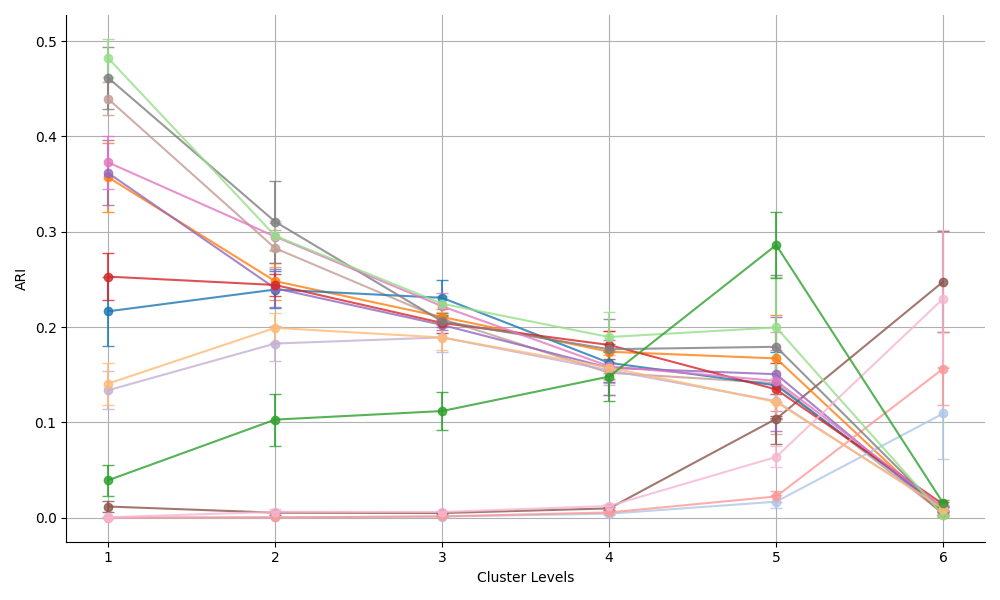
\includegraphics[width=\linewidth]{ARI_plot_None_hierarchy_t1.0_maxsub3_depth5_synonymsNone_noiseNone_random.png}
            \caption*{Deep datasets}
        \end{subfigure}
        \hfill
        \begin{subfigure}[t]{0.49\linewidth}
            \centering
            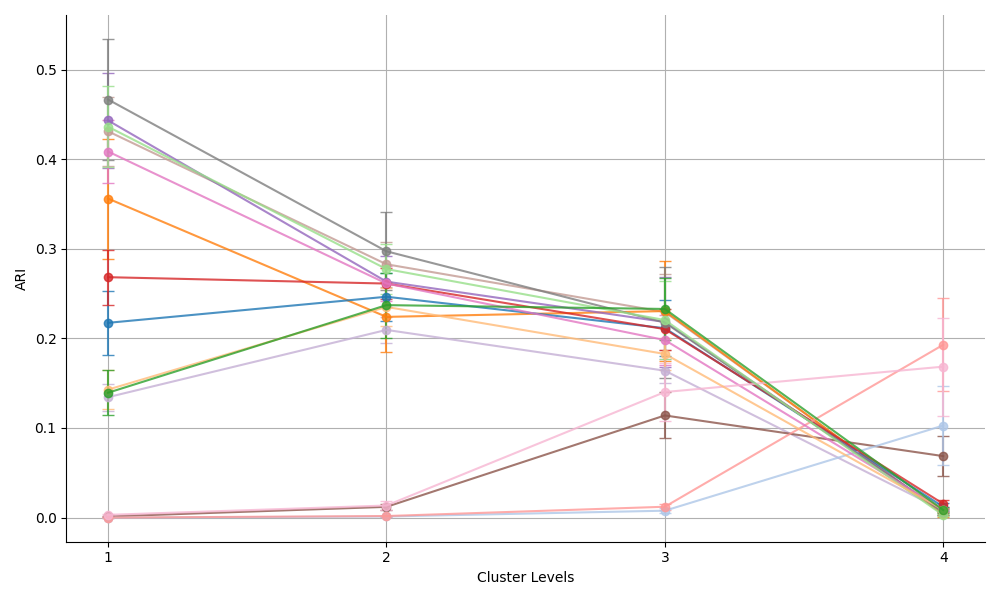
\includegraphics[width=\linewidth]{ARI_plot_None_hierarchy_t1.0_maxsub5_depth3_synonymsNone_noiseNone_random.png}
            \caption*{Shallow datasets}
        \end{subfigure}
    \end{minipage}
    \hfill
    \begin{minipage}[t]{0.25\linewidth}
        \centering
        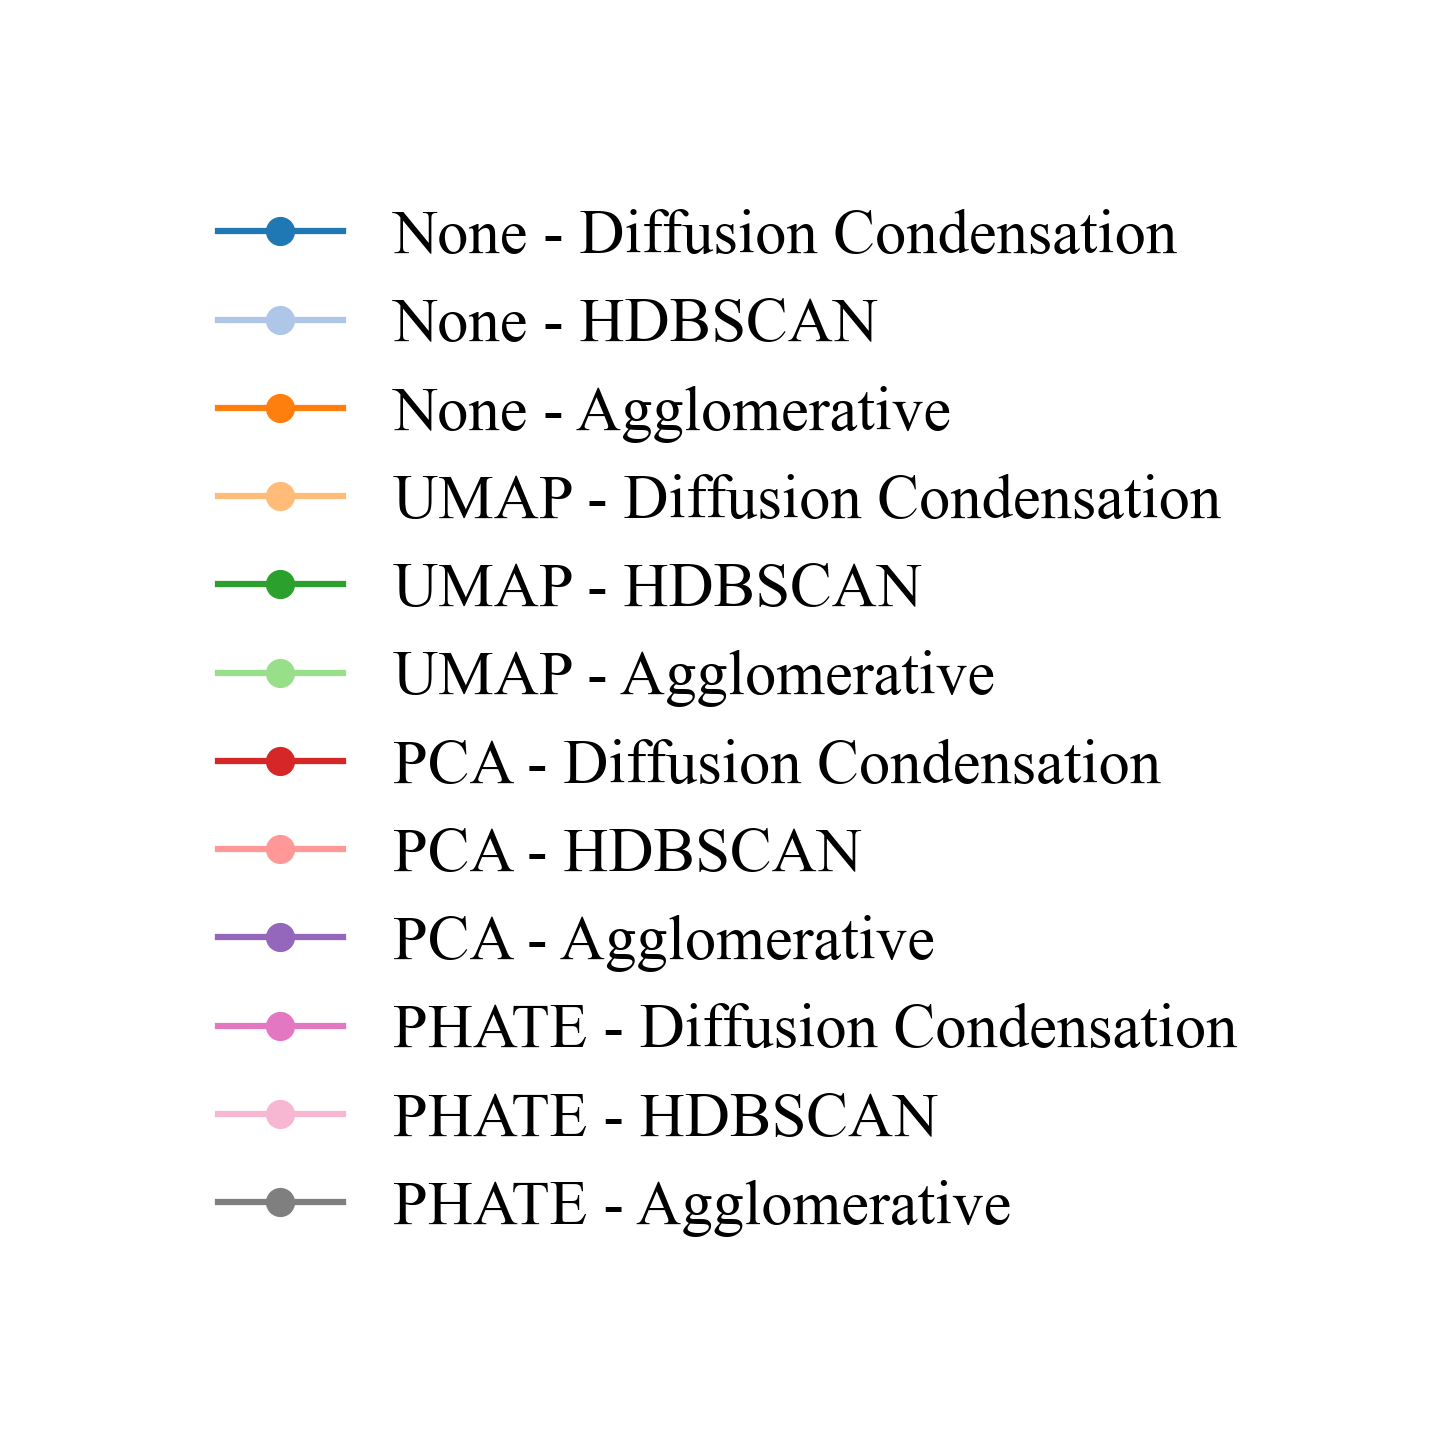
\includegraphics[width=\linewidth]{legend_None_t1.0_maxsub3_depth5_noiseNone_random.png}
    \end{minipage}
    \caption{Line plot of performance at each cluster level averaged across deep and shallow generated datasets. Lower numbers on the x-axis correspond to coarser scales (i.e., fewer clusters). \textit{None} means no dimensionality reduction. Bars represent standard error.}
    \label{fig:ARI-combined}
\end{figure*}